% Options for packages loaded elsewhere
\PassOptionsToPackage{unicode}{hyperref}
\PassOptionsToPackage{hyphens}{url}
%
\documentclass[
]{article}
\usepackage{lmodern}
\usepackage{amssymb,amsmath}
\usepackage{ifxetex,ifluatex}
\ifnum 0\ifxetex 1\fi\ifluatex 1\fi=0 % if pdftex
  \usepackage[T1]{fontenc}
  \usepackage[utf8]{inputenc}
  \usepackage{textcomp} % provide euro and other symbols
\else % if luatex or xetex
  \usepackage{unicode-math}
  \defaultfontfeatures{Scale=MatchLowercase}
  \defaultfontfeatures[\rmfamily]{Ligatures=TeX,Scale=1}
\fi
% Use upquote if available, for straight quotes in verbatim environments
\IfFileExists{upquote.sty}{\usepackage{upquote}}{}
\IfFileExists{microtype.sty}{% use microtype if available
  \usepackage[]{microtype}
  \UseMicrotypeSet[protrusion]{basicmath} % disable protrusion for tt fonts
}{}
\makeatletter
\@ifundefined{KOMAClassName}{% if non-KOMA class
  \IfFileExists{parskip.sty}{%
    \usepackage{parskip}
  }{% else
    \setlength{\parindent}{0pt}
    \setlength{\parskip}{6pt plus 2pt minus 1pt}}
}{% if KOMA class
  \KOMAoptions{parskip=half}}
\makeatother
\usepackage{xcolor}
\IfFileExists{xurl.sty}{\usepackage{xurl}}{} % add URL line breaks if available
\IfFileExists{bookmark.sty}{\usepackage{bookmark}}{\usepackage{hyperref}}
\hypersetup{
  pdftitle={4.13},
  pdfauthor={Greg Matesi},
  hidelinks,
  pdfcreator={LaTeX via pandoc}}
\urlstyle{same} % disable monospaced font for URLs
\usepackage[margin=1in]{geometry}
\usepackage{color}
\usepackage{fancyvrb}
\newcommand{\VerbBar}{|}
\newcommand{\VERB}{\Verb[commandchars=\\\{\}]}
\DefineVerbatimEnvironment{Highlighting}{Verbatim}{commandchars=\\\{\}}
% Add ',fontsize=\small' for more characters per line
\usepackage{framed}
\definecolor{shadecolor}{RGB}{248,248,248}
\newenvironment{Shaded}{\begin{snugshade}}{\end{snugshade}}
\newcommand{\AlertTok}[1]{\textcolor[rgb]{0.94,0.16,0.16}{#1}}
\newcommand{\AnnotationTok}[1]{\textcolor[rgb]{0.56,0.35,0.01}{\textbf{\textit{#1}}}}
\newcommand{\AttributeTok}[1]{\textcolor[rgb]{0.77,0.63,0.00}{#1}}
\newcommand{\BaseNTok}[1]{\textcolor[rgb]{0.00,0.00,0.81}{#1}}
\newcommand{\BuiltInTok}[1]{#1}
\newcommand{\CharTok}[1]{\textcolor[rgb]{0.31,0.60,0.02}{#1}}
\newcommand{\CommentTok}[1]{\textcolor[rgb]{0.56,0.35,0.01}{\textit{#1}}}
\newcommand{\CommentVarTok}[1]{\textcolor[rgb]{0.56,0.35,0.01}{\textbf{\textit{#1}}}}
\newcommand{\ConstantTok}[1]{\textcolor[rgb]{0.00,0.00,0.00}{#1}}
\newcommand{\ControlFlowTok}[1]{\textcolor[rgb]{0.13,0.29,0.53}{\textbf{#1}}}
\newcommand{\DataTypeTok}[1]{\textcolor[rgb]{0.13,0.29,0.53}{#1}}
\newcommand{\DecValTok}[1]{\textcolor[rgb]{0.00,0.00,0.81}{#1}}
\newcommand{\DocumentationTok}[1]{\textcolor[rgb]{0.56,0.35,0.01}{\textbf{\textit{#1}}}}
\newcommand{\ErrorTok}[1]{\textcolor[rgb]{0.64,0.00,0.00}{\textbf{#1}}}
\newcommand{\ExtensionTok}[1]{#1}
\newcommand{\FloatTok}[1]{\textcolor[rgb]{0.00,0.00,0.81}{#1}}
\newcommand{\FunctionTok}[1]{\textcolor[rgb]{0.00,0.00,0.00}{#1}}
\newcommand{\ImportTok}[1]{#1}
\newcommand{\InformationTok}[1]{\textcolor[rgb]{0.56,0.35,0.01}{\textbf{\textit{#1}}}}
\newcommand{\KeywordTok}[1]{\textcolor[rgb]{0.13,0.29,0.53}{\textbf{#1}}}
\newcommand{\NormalTok}[1]{#1}
\newcommand{\OperatorTok}[1]{\textcolor[rgb]{0.81,0.36,0.00}{\textbf{#1}}}
\newcommand{\OtherTok}[1]{\textcolor[rgb]{0.56,0.35,0.01}{#1}}
\newcommand{\PreprocessorTok}[1]{\textcolor[rgb]{0.56,0.35,0.01}{\textit{#1}}}
\newcommand{\RegionMarkerTok}[1]{#1}
\newcommand{\SpecialCharTok}[1]{\textcolor[rgb]{0.00,0.00,0.00}{#1}}
\newcommand{\SpecialStringTok}[1]{\textcolor[rgb]{0.31,0.60,0.02}{#1}}
\newcommand{\StringTok}[1]{\textcolor[rgb]{0.31,0.60,0.02}{#1}}
\newcommand{\VariableTok}[1]{\textcolor[rgb]{0.00,0.00,0.00}{#1}}
\newcommand{\VerbatimStringTok}[1]{\textcolor[rgb]{0.31,0.60,0.02}{#1}}
\newcommand{\WarningTok}[1]{\textcolor[rgb]{0.56,0.35,0.01}{\textbf{\textit{#1}}}}
\usepackage{graphicx,grffile}
\makeatletter
\def\maxwidth{\ifdim\Gin@nat@width>\linewidth\linewidth\else\Gin@nat@width\fi}
\def\maxheight{\ifdim\Gin@nat@height>\textheight\textheight\else\Gin@nat@height\fi}
\makeatother
% Scale images if necessary, so that they will not overflow the page
% margins by default, and it is still possible to overwrite the defaults
% using explicit options in \includegraphics[width, height, ...]{}
\setkeys{Gin}{width=\maxwidth,height=\maxheight,keepaspectratio}
% Set default figure placement to htbp
\makeatletter
\def\fps@figure{htbp}
\makeatother
\setlength{\emergencystretch}{3em} % prevent overfull lines
\providecommand{\tightlist}{%
  \setlength{\itemsep}{0pt}\setlength{\parskip}{0pt}}
\setcounter{secnumdepth}{-\maxdimen} % remove section numbering

\title{4.13}
\author{Greg Matesi}
\date{July 5, 2020}

\begin{document}
\maketitle

\hypertarget{load-the-data}{%
\section{Load the data}\label{load-the-data}}

\begin{Shaded}
\begin{Highlighting}[]
\KeywordTok{options}\NormalTok{(}\DataTypeTok{digits=}\DecValTok{4}\NormalTok{)}

\CommentTok{# MASS library for the Boston data and lda()}
\KeywordTok{library}\NormalTok{(MASS)}

\KeywordTok{attach}\NormalTok{(Boston)}

\CommentTok{# class library for knn()}
\KeywordTok{library}\NormalTok{(class)}

\CommentTok{# Initial look at the data}
\KeywordTok{dim}\NormalTok{(Boston)}
\end{Highlighting}
\end{Shaded}

\begin{verbatim}
## [1] 506  14
\end{verbatim}

\begin{Shaded}
\begin{Highlighting}[]
\KeywordTok{head}\NormalTok{(Boston)}
\end{Highlighting}
\end{Shaded}

\begin{verbatim}
##      crim zn indus chas   nox    rm  age   dis rad tax ptratio black lstat medv
## 1 0.00632 18  2.31    0 0.538 6.575 65.2 4.090   1 296    15.3 396.9  4.98 24.0
## 2 0.02731  0  7.07    0 0.469 6.421 78.9 4.967   2 242    17.8 396.9  9.14 21.6
## 3 0.02729  0  7.07    0 0.469 7.185 61.1 4.967   2 242    17.8 392.8  4.03 34.7
## 4 0.03237  0  2.18    0 0.458 6.998 45.8 6.062   3 222    18.7 394.6  2.94 33.4
## 5 0.06905  0  2.18    0 0.458 7.147 54.2 6.062   3 222    18.7 396.9  5.33 36.2
## 6 0.02985  0  2.18    0 0.458 6.430 58.7 6.062   3 222    18.7 394.1  5.21 28.7
\end{verbatim}

\begin{Shaded}
\begin{Highlighting}[]
\KeywordTok{summary}\NormalTok{(crim)}
\end{Highlighting}
\end{Shaded}

\begin{verbatim}
##    Min. 1st Qu.  Median    Mean 3rd Qu.    Max. 
##    0.01    0.08    0.26    3.61    3.68   88.98
\end{verbatim}

\hypertarget{make-dummy-variable}{%
\section{Make dummy variable}\label{make-dummy-variable}}

Make a dummy variable called highcrime. This variable will be ``TRUE''
if crim is greater than it's median. And it will be ``FALSE'' if crim is
less than it's median.

\begin{Shaded}
\begin{Highlighting}[]
\NormalTok{med.crim <-}\StringTok{ }\KeywordTok{median}\NormalTok{(crim)}
\NormalTok{Boston}\OperatorTok{$}\NormalTok{highcrime <-}\StringTok{ }\NormalTok{Boston}\OperatorTok{$}\NormalTok{crim }\OperatorTok{>}\StringTok{ }\NormalTok{med.crim}

\CommentTok{# remove the crim variable. It has been replaced with highcrime}
\NormalTok{Boston <-}\StringTok{ }\NormalTok{Boston[,}\OperatorTok{-}\KeywordTok{c}\NormalTok{(}\DecValTok{1}\NormalTok{)]}
\KeywordTok{attach}\NormalTok{(Boston)}
\end{Highlighting}
\end{Shaded}

\begin{verbatim}
## The following objects are masked from Boston (pos = 4):
## 
##     age, black, chas, dis, indus, lstat, medv, nox, ptratio, rad, rm,
##     tax, zn
\end{verbatim}

\begin{Shaded}
\begin{Highlighting}[]
\KeywordTok{names}\NormalTok{(Boston)}
\end{Highlighting}
\end{Shaded}

\begin{verbatim}
##  [1] "zn"        "indus"     "chas"      "nox"       "rm"        "age"      
##  [7] "dis"       "rad"       "tax"       "ptratio"   "black"     "lstat"    
## [13] "medv"      "highcrime"
\end{verbatim}

\begin{Shaded}
\begin{Highlighting}[]
\KeywordTok{dim}\NormalTok{(Boston)}
\end{Highlighting}
\end{Shaded}

\begin{verbatim}
## [1] 506  14
\end{verbatim}

\begin{Shaded}
\begin{Highlighting}[]
\CommentTok{# there should be an equal amount of observations above and below the mean}
\KeywordTok{summary}\NormalTok{(Boston}\OperatorTok{$}\NormalTok{highcrime)}
\end{Highlighting}
\end{Shaded}

\begin{verbatim}
##    Mode   FALSE    TRUE 
## logical     253     253
\end{verbatim}

\begin{Shaded}
\begin{Highlighting}[]
\CommentTok{# Looking at the highcrime variable.}
\KeywordTok{cor}\NormalTok{(Boston)}
\end{Highlighting}
\end{Shaded}

\begin{verbatim}
##                zn    indus      chas     nox       rm      age      dis
## zn         1.0000 -0.53383 -0.042697 -0.5166  0.31199 -0.56954  0.66441
## indus     -0.5338  1.00000  0.062938  0.7637 -0.39168  0.64478 -0.70803
## chas      -0.0427  0.06294  1.000000  0.0912  0.09125  0.08652 -0.09918
## nox       -0.5166  0.76365  0.091203  1.0000 -0.30219  0.73147 -0.76923
## rm         0.3120 -0.39168  0.091251 -0.3022  1.00000 -0.24026  0.20525
## age       -0.5695  0.64478  0.086518  0.7315 -0.24026  1.00000 -0.74788
## dis        0.6644 -0.70803 -0.099176 -0.7692  0.20525 -0.74788  1.00000
## rad       -0.3119  0.59513 -0.007368  0.6114 -0.20985  0.45602 -0.49459
## tax       -0.3146  0.72076 -0.035587  0.6680 -0.29205  0.50646 -0.53443
## ptratio   -0.3917  0.38325 -0.121515  0.1889 -0.35550  0.26152 -0.23247
## black      0.1755 -0.35698  0.048788 -0.3801  0.12807 -0.27353  0.29151
## lstat     -0.4130  0.60380 -0.053929  0.5909 -0.61381  0.60234 -0.49700
## medv       0.3604 -0.48373  0.175260 -0.4273  0.69536 -0.37695  0.24993
## highcrime -0.4362  0.60326  0.070097  0.7232 -0.15637  0.61394 -0.61634
##                 rad      tax ptratio    black    lstat    medv highcrime
## zn        -0.311948 -0.31456 -0.3917  0.17552 -0.41299  0.3604   -0.4362
## indus      0.595129  0.72076  0.3832 -0.35698  0.60380 -0.4837    0.6033
## chas      -0.007368 -0.03559 -0.1215  0.04879 -0.05393  0.1753    0.0701
## nox        0.611441  0.66802  0.1889 -0.38005  0.59088 -0.4273    0.7232
## rm        -0.209847 -0.29205 -0.3555  0.12807 -0.61381  0.6954   -0.1564
## age        0.456022  0.50646  0.2615 -0.27353  0.60234 -0.3770    0.6139
## dis       -0.494588 -0.53443 -0.2325  0.29151 -0.49700  0.2499   -0.6163
## rad        1.000000  0.91023  0.4647 -0.44441  0.48868 -0.3816    0.6198
## tax        0.910228  1.00000  0.4609 -0.44181  0.54399 -0.4685    0.6087
## ptratio    0.464741  0.46085  1.0000 -0.17738  0.37404 -0.5078    0.2536
## black     -0.444413 -0.44181 -0.1774  1.00000 -0.36609  0.3335   -0.3512
## lstat      0.488676  0.54399  0.3740 -0.36609  1.00000 -0.7377    0.4533
## medv      -0.381626 -0.46854 -0.5078  0.33346 -0.73766  1.0000   -0.2630
## highcrime  0.619786  0.60874  0.2536 -0.35121  0.45326 -0.2630    1.0000
\end{verbatim}

\begin{Shaded}
\begin{Highlighting}[]
\KeywordTok{plot}\NormalTok{(crim)}
\KeywordTok{abline}\NormalTok{(}\DataTypeTok{h=}\NormalTok{med.crim)}
\end{Highlighting}
\end{Shaded}

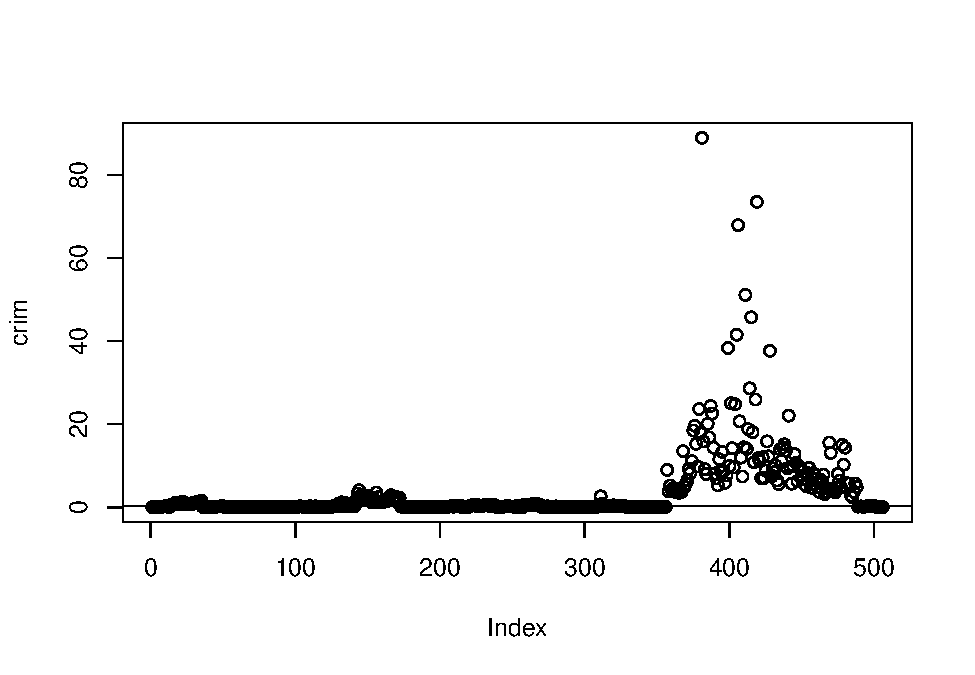
\includegraphics{4-13_files/figure-latex/unnamed-chunk-3-1.pdf}

\begin{Shaded}
\begin{Highlighting}[]
\KeywordTok{plot}\NormalTok{(highcrime)}
\end{Highlighting}
\end{Shaded}

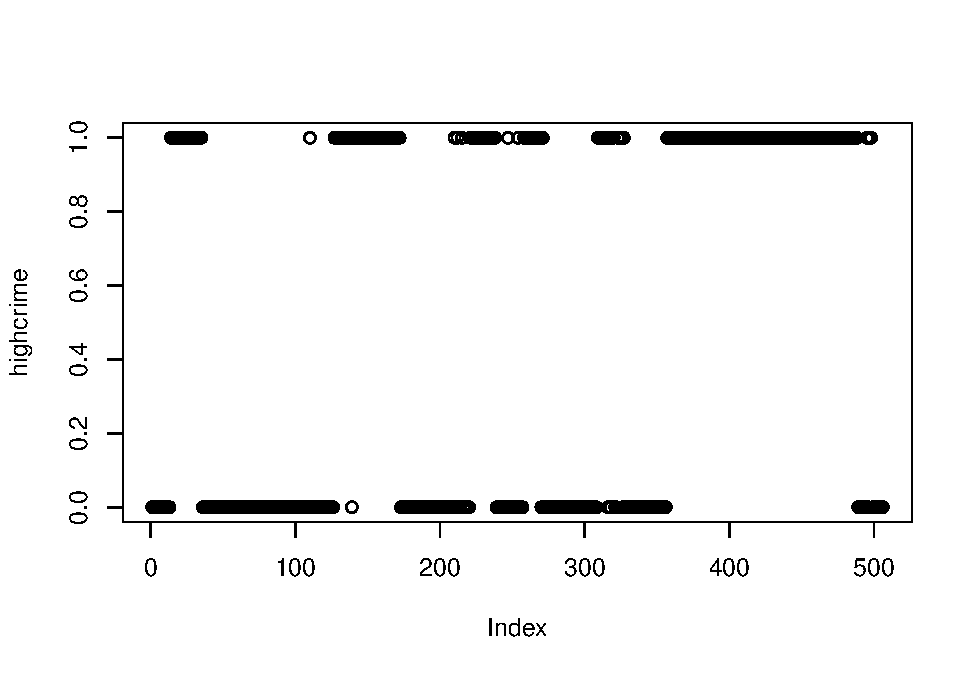
\includegraphics{4-13_files/figure-latex/unnamed-chunk-3-2.pdf}

\hypertarget{subset}{%
\section{Subset}\label{subset}}

Subset the data into a training set and a test set. The variable
subsetfrac can be adjusted to allow for a larger or smaller fraction to
be used as a test set.

\begin{Shaded}
\begin{Highlighting}[]
\NormalTok{subsetfrac <-}\StringTok{ }\DecValTok{1}\OperatorTok{/}\DecValTok{3}
\NormalTok{train.index <-}\StringTok{ }\KeywordTok{sample}\NormalTok{(}\KeywordTok{dim}\NormalTok{(Boston)[}\DecValTok{1}\NormalTok{], (}\DecValTok{1}\OperatorTok{-}\NormalTok{subsetfrac)}\OperatorTok{*}\KeywordTok{dim}\NormalTok{(Boston)[}\DecValTok{1}\NormalTok{] )}

\NormalTok{Boston.test <-}\StringTok{ }\NormalTok{Boston[}\OperatorTok{-}\KeywordTok{c}\NormalTok{(train.index),]}
\NormalTok{Boston.train <-}\StringTok{ }\NormalTok{Boston[}\KeywordTok{c}\NormalTok{(train.index),]}

\NormalTok{highcrime.test <-}\StringTok{ }\NormalTok{highcrime[}\OperatorTok{-}\KeywordTok{c}\NormalTok{(train.index)]}
\end{Highlighting}
\end{Shaded}

\hypertarget{logistic}{%
\section{Logistic}\label{logistic}}

Fit a logistic regression model using nox, ptratio, chas, and indus as
variables.

\begin{Shaded}
\begin{Highlighting}[]
\NormalTok{glm.fit <-}\StringTok{ }\KeywordTok{glm}\NormalTok{(highcrime}\OperatorTok{~}\NormalTok{nox}\OperatorTok{+}\NormalTok{ptratio}\OperatorTok{+}\NormalTok{chas}\OperatorTok{+}\NormalTok{indus,}
               \DataTypeTok{data =}\NormalTok{ Boston.train,}
               \DataTypeTok{family =}\NormalTok{ binomial)}

\KeywordTok{coef}\NormalTok{(glm.fit)}
\end{Highlighting}
\end{Shaded}

\begin{verbatim}
## (Intercept)         nox     ptratio        chas       indus 
##   -19.76394    34.45769     0.09389     0.97389    -0.06036
\end{verbatim}

\begin{Shaded}
\begin{Highlighting}[]
\KeywordTok{summary}\NormalTok{(glm.fit)}
\end{Highlighting}
\end{Shaded}

\begin{verbatim}
## 
## Call:
## glm(formula = highcrime ~ nox + ptratio + chas + indus, family = binomial, 
##     data = Boston.train)
## 
## Deviance Residuals: 
##    Min      1Q  Median      3Q     Max  
## -2.233  -0.376  -0.120   0.415   2.647  
## 
## Coefficients:
##             Estimate Std. Error z value Pr(>|z|)    
## (Intercept) -19.7639     3.0335   -6.52  7.3e-11 ***
## nox          34.4577     5.1486    6.69  2.2e-11 ***
## ptratio       0.0939     0.0933    1.01     0.31    
## chas          0.9739     0.6568    1.48     0.14    
## indus        -0.0604     0.0450   -1.34     0.18    
## ---
## Signif. codes:  0 '***' 0.001 '**' 0.01 '*' 0.05 '.' 0.1 ' ' 1
## 
## (Dispersion parameter for binomial family taken to be 1)
## 
##     Null deviance: 467.18  on 336  degrees of freedom
## Residual deviance: 207.18  on 332  degrees of freedom
## AIC: 217.2
## 
## Number of Fisher Scoring iterations: 7
\end{verbatim}

Predict the probability that a neighborhood will have a high crime rate.

\begin{Shaded}
\begin{Highlighting}[]
\NormalTok{glm.probs <-}\StringTok{ }\KeywordTok{predict}\NormalTok{(glm.fit,}
                     \DataTypeTok{newdata =}\NormalTok{ Boston.test,}
                     \DataTypeTok{type =} \StringTok{"response"}\NormalTok{)}
\NormalTok{glm.probs[}\DecValTok{1}\OperatorTok{:}\DecValTok{10}\NormalTok{]}
\end{Highlighting}
\end{Shaded}

\begin{verbatim}
##       4       5       9      10      12      14      15      16      17      19 
## 0.08643 0.08643 0.31953 0.31953 0.31953 0.56335 0.56335 0.56335 0.56335 0.56335
\end{verbatim}

Predict whether a neighborhood in the test set will have a high crime
rate probability of greater or less than 50\%

\begin{Shaded}
\begin{Highlighting}[]
\NormalTok{probability <-}\StringTok{ }\FloatTok{.5}
\NormalTok{glm.pred <-}\StringTok{ }\KeywordTok{rep}\NormalTok{(}\OtherTok{FALSE}\NormalTok{, }\KeywordTok{length}\NormalTok{(highcrime.test))}
\NormalTok{glm.pred[glm.probs }\OperatorTok{>}\StringTok{ }\NormalTok{probability]=}\OtherTok{TRUE}
\end{Highlighting}
\end{Shaded}

Assess the model.

\begin{Shaded}
\begin{Highlighting}[]
\NormalTok{glm.table <-}\StringTok{ }\KeywordTok{table}\NormalTok{(glm.pred,highcrime.test)}
\NormalTok{glm.table}
\end{Highlighting}
\end{Shaded}

\begin{verbatim}
##         highcrime.test
## glm.pred FALSE TRUE
##    FALSE    70   12
##    TRUE     14   73
\end{verbatim}

\begin{Shaded}
\begin{Highlighting}[]
\KeywordTok{mean}\NormalTok{(glm.pred}\OperatorTok{==}\NormalTok{highcrime.test)}
\end{Highlighting}
\end{Shaded}

\begin{verbatim}
## [1] 0.8462
\end{verbatim}

\begin{Shaded}
\begin{Highlighting}[]
\NormalTok{(glm.table[}\DecValTok{1}\NormalTok{,}\DecValTok{1}\NormalTok{]}\OperatorTok{+}\NormalTok{glm.table[}\DecValTok{2}\NormalTok{,}\DecValTok{2}\NormalTok{]) }\OperatorTok{/}\StringTok{ }\KeywordTok{length}\NormalTok{(highcrime.test)}
\end{Highlighting}
\end{Shaded}

\begin{verbatim}
## [1] 0.8462
\end{verbatim}

\hypertarget{lda}{%
\section{LDA}\label{lda}}

Fit linear discriminate analysis model on the Boston data.

\begin{Shaded}
\begin{Highlighting}[]
\NormalTok{lda.fit <-}\StringTok{ }\KeywordTok{lda}\NormalTok{(highcrime}\OperatorTok{~}\NormalTok{nox}\OperatorTok{+}\NormalTok{ptratio}\OperatorTok{+}\NormalTok{chas}\OperatorTok{+}\NormalTok{indus, }
               \DataTypeTok{data=}\NormalTok{Boston, }
               \DataTypeTok{subset=}\NormalTok{train.index)}
\NormalTok{lda.fit}
\end{Highlighting}
\end{Shaded}

\begin{verbatim}
## Call:
## lda(highcrime ~ nox + ptratio + chas + indus, data = Boston, 
##     subset = train.index)
## 
## Prior probabilities of groups:
##  FALSE   TRUE 
## 0.5015 0.4985 
## 
## Group means:
##          nox ptratio    chas  indus
## FALSE 0.4716   18.03 0.05325  6.947
## TRUE  0.6388   18.91 0.08333 15.282
## 
## Coefficients of linear discriminants:
##              LD1
## nox     10.77092
## ptratio  0.08476
## chas     0.13859
## indus    0.03436
\end{verbatim}

\begin{Shaded}
\begin{Highlighting}[]
\KeywordTok{plot}\NormalTok{(lda.fit)}
\end{Highlighting}
\end{Shaded}

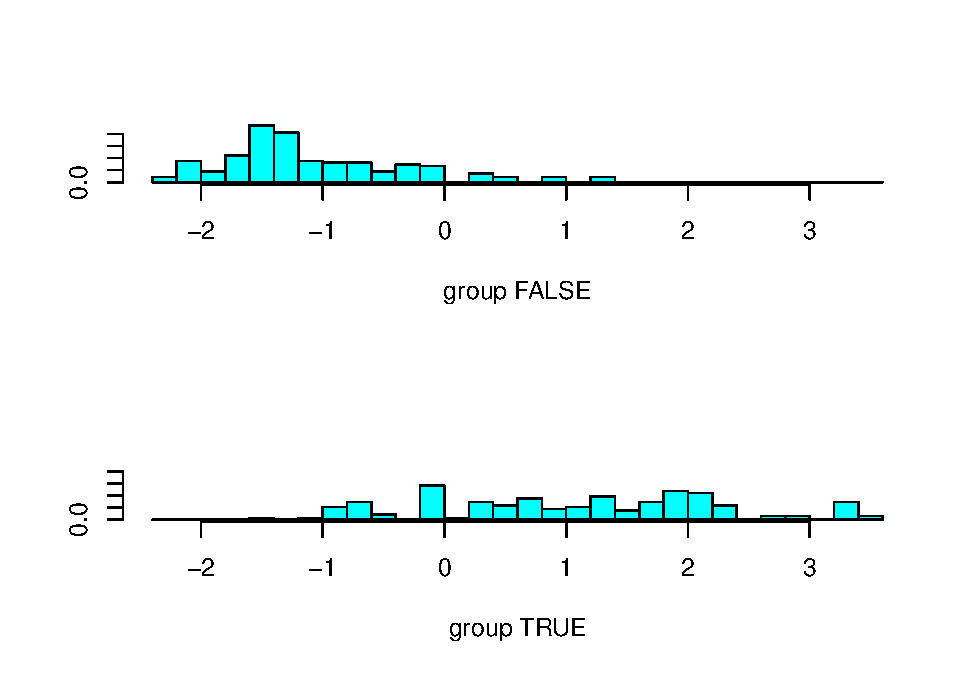
\includegraphics{4-13_files/figure-latex/unnamed-chunk-9-1.pdf}

Use the lda model to predict whether neighborhoods in the test set will
have a high crime rate.

\begin{Shaded}
\begin{Highlighting}[]
\NormalTok{lda.pred=}\KeywordTok{predict}\NormalTok{(lda.fit, Boston.test)}
\KeywordTok{names}\NormalTok{(lda.pred)}
\end{Highlighting}
\end{Shaded}

\begin{verbatim}
## [1] "class"     "posterior" "x"
\end{verbatim}

\begin{Shaded}
\begin{Highlighting}[]
\NormalTok{lda.class <-}\StringTok{ }\NormalTok{lda.pred}\OperatorTok{$}\NormalTok{class}
\NormalTok{lda.table <-}\StringTok{ }\KeywordTok{table}\NormalTok{(lda.class, highcrime.test)}
\NormalTok{lda.table}
\end{Highlighting}
\end{Shaded}

\begin{verbatim}
##          highcrime.test
## lda.class FALSE TRUE
##     FALSE    76   22
##     TRUE      8   63
\end{verbatim}

\begin{Shaded}
\begin{Highlighting}[]
\KeywordTok{mean}\NormalTok{(lda.class}\OperatorTok{==}\NormalTok{highcrime.test)}
\end{Highlighting}
\end{Shaded}

\begin{verbatim}
## [1] 0.8225
\end{verbatim}

\begin{Shaded}
\begin{Highlighting}[]
\NormalTok{(lda.table[}\DecValTok{1}\NormalTok{,}\DecValTok{1}\NormalTok{]}\OperatorTok{+}\NormalTok{lda.table[}\DecValTok{2}\NormalTok{,}\DecValTok{2}\NormalTok{]) }\OperatorTok{/}\StringTok{ }\KeywordTok{length}\NormalTok{(highcrime.test)}
\end{Highlighting}
\end{Shaded}

\begin{verbatim}
## [1] 0.8225
\end{verbatim}

\hypertarget{knn}{%
\section{KNN}\label{knn}}

\begin{Shaded}
\begin{Highlighting}[]
\NormalTok{variable.list <-}\StringTok{ }\KeywordTok{c}\NormalTok{(}\StringTok{"nox"}\NormalTok{, }\StringTok{"ptratio"}\NormalTok{, }\StringTok{"chas"}\NormalTok{, }\StringTok{"indus"}\NormalTok{)}
\NormalTok{train.x <-}\StringTok{ }\NormalTok{Boston.train[,variable.list]}
\NormalTok{test.x  <-}\StringTok{ }\NormalTok{Boston.test[,variable.list]}
\NormalTok{train.highcrime <-}\StringTok{ }\KeywordTok{cbind}\NormalTok{(Boston.train}\OperatorTok{$}\NormalTok{highcrime)}
\end{Highlighting}
\end{Shaded}

\begin{Shaded}
\begin{Highlighting}[]
\NormalTok{numk =}\StringTok{ }\DecValTok{1}
\NormalTok{knn.pred <-}\StringTok{ }\KeywordTok{knn}\NormalTok{(train.x, }
\NormalTok{                test.x,}
\NormalTok{                train.highcrime,}
                \DataTypeTok{k=}\NormalTok{numk)}

\NormalTok{knn.table <-}\StringTok{ }\KeywordTok{table}\NormalTok{(knn.pred,highcrime.test)}
\NormalTok{knn.table}
\end{Highlighting}
\end{Shaded}

\begin{verbatim}
##         highcrime.test
## knn.pred FALSE TRUE
##    FALSE    77    3
##    TRUE      7   82
\end{verbatim}

\begin{Shaded}
\begin{Highlighting}[]
\NormalTok{(knn.table[}\DecValTok{1}\NormalTok{,}\DecValTok{1}\NormalTok{]}\OperatorTok{+}\NormalTok{knn.table[}\DecValTok{2}\NormalTok{,}\DecValTok{2}\NormalTok{])}\OperatorTok{/}\KeywordTok{length}\NormalTok{(highcrime.test)}
\end{Highlighting}
\end{Shaded}

\begin{verbatim}
## [1] 0.9408
\end{verbatim}

\begin{Shaded}
\begin{Highlighting}[]
\KeywordTok{mean}\NormalTok{(knn.pred }\OperatorTok{==}\StringTok{ }\NormalTok{highcrime.test)}
\end{Highlighting}
\end{Shaded}

\begin{verbatim}
## [1] 0.9408
\end{verbatim}

\hypertarget{analysis}{%
\section{Analysis}\label{analysis}}

We see that lda and logistic regression predicts equally well on the
test set. Each of these two models predict correctly for
\textasciitilde85\% of the observations. The third model, k nearest
neighbors with k=1 outperforms them in this respect. It predicts
correctly on the test set \textasciitilde95\% of the time.

\hypertarget{sensitivity}{%
\subsection{Sensitivity}\label{sensitivity}}

The true positive rate of these three methods is examined below.

\begin{Shaded}
\begin{Highlighting}[]
\NormalTok{glm.table[}\DecValTok{2}\NormalTok{,}\DecValTok{2}\NormalTok{]}\OperatorTok{/}\NormalTok{(glm.table[}\DecValTok{2}\NormalTok{,}\DecValTok{2}\NormalTok{]}\OperatorTok{+}\NormalTok{glm.table[}\DecValTok{1}\NormalTok{,}\DecValTok{2}\NormalTok{])}
\end{Highlighting}
\end{Shaded}

\begin{verbatim}
## [1] 0.8588
\end{verbatim}

\begin{Shaded}
\begin{Highlighting}[]
\NormalTok{lda.table[}\DecValTok{2}\NormalTok{,}\DecValTok{2}\NormalTok{]}\OperatorTok{/}\NormalTok{(lda.table[}\DecValTok{2}\NormalTok{,}\DecValTok{2}\NormalTok{]}\OperatorTok{+}\NormalTok{lda.table[}\DecValTok{1}\NormalTok{,}\DecValTok{2}\NormalTok{])}
\end{Highlighting}
\end{Shaded}

\begin{verbatim}
## [1] 0.7412
\end{verbatim}

\begin{Shaded}
\begin{Highlighting}[]
\NormalTok{knn.table[}\DecValTok{2}\NormalTok{,}\DecValTok{2}\NormalTok{]}\OperatorTok{/}\NormalTok{(knn.table[}\DecValTok{2}\NormalTok{,}\DecValTok{2}\NormalTok{]}\OperatorTok{+}\NormalTok{knn.table[}\DecValTok{1}\NormalTok{,}\DecValTok{2}\NormalTok{])}
\end{Highlighting}
\end{Shaded}

\begin{verbatim}
## [1] 0.9647
\end{verbatim}

Knn with k=1 outperforms both of the other two models in sensitivity,
the ability to correctly predict a true high crime rate. \#\#
Specificity

The true negative rate for the three models is examined blow.

\begin{Shaded}
\begin{Highlighting}[]
\NormalTok{glm.table[}\DecValTok{1}\NormalTok{,}\DecValTok{1}\NormalTok{]}\OperatorTok{/}\NormalTok{(glm.table[}\DecValTok{1}\NormalTok{,}\DecValTok{1}\NormalTok{]}\OperatorTok{+}\NormalTok{glm.table[}\DecValTok{2}\NormalTok{,}\DecValTok{1}\NormalTok{])}
\end{Highlighting}
\end{Shaded}

\begin{verbatim}
## [1] 0.8333
\end{verbatim}

\begin{Shaded}
\begin{Highlighting}[]
\NormalTok{lda.table[}\DecValTok{1}\NormalTok{,}\DecValTok{1}\NormalTok{]}\OperatorTok{/}\NormalTok{(lda.table[}\DecValTok{1}\NormalTok{,}\DecValTok{1}\NormalTok{]}\OperatorTok{+}\NormalTok{lda.table[}\DecValTok{2}\NormalTok{,}\DecValTok{1}\NormalTok{])}
\end{Highlighting}
\end{Shaded}

\begin{verbatim}
## [1] 0.9048
\end{verbatim}

\begin{Shaded}
\begin{Highlighting}[]
\NormalTok{knn.table[}\DecValTok{1}\NormalTok{,}\DecValTok{1}\NormalTok{]}\OperatorTok{/}\NormalTok{(knn.table[}\DecValTok{1}\NormalTok{,}\DecValTok{1}\NormalTok{]}\OperatorTok{+}\NormalTok{knn.table[}\DecValTok{2}\NormalTok{,}\DecValTok{1}\NormalTok{])}
\end{Highlighting}
\end{Shaded}

\begin{verbatim}
## [1] 0.9167
\end{verbatim}

We see that knn with k=1 also outperforms the other two models in
sensitivity. The ability to correctly predict a low crime rate.

\end{document}
